\begin{figure}[htbp]
\centering
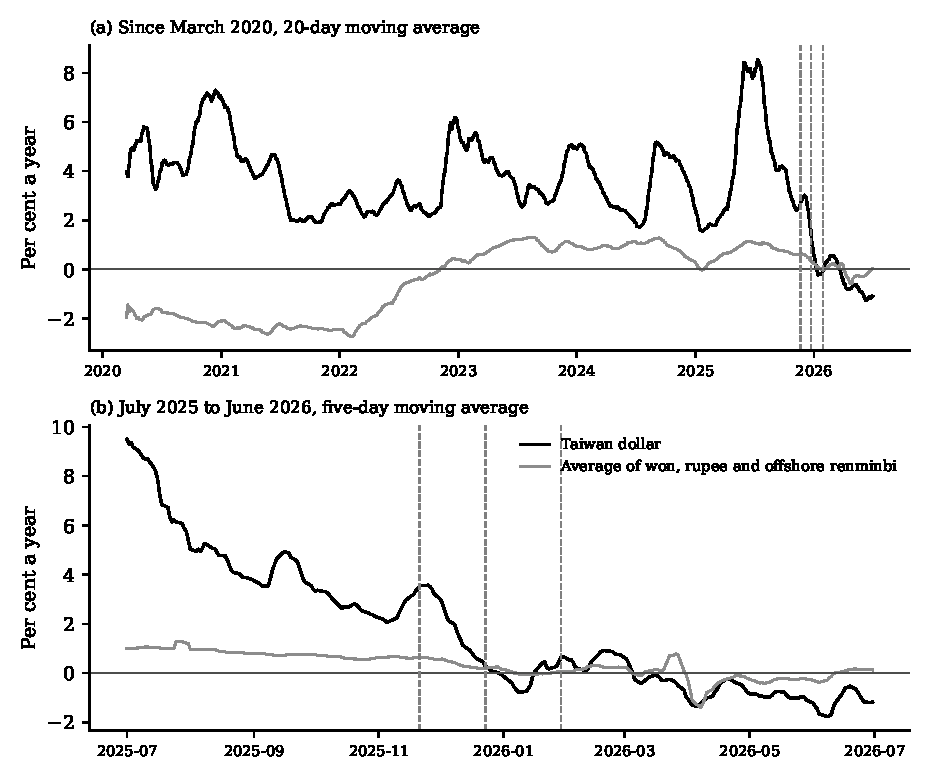
\includegraphics[width=0.86\textwidth]{results/fig_futures.pdf}
\caption{Dollar's three-month forward discount implied by Singapore Exchange currency futures. Annualised difference between the settlement prices of the nearest and the fourth contract; positive values are a forward discount of the dollar, negative values a premium. Dashed lines mark the industry's proposal (21 November 2025), the draft amendment (23 December 2025) and the issuance of the amendment (29 January 2026). Source: Singapore Exchange.}\label{fig:futures}
\end{figure}

\begin{table}[htbp]
\centering
\small
\begin{threeparttable}
\caption{Forward discount implied by Taiwan-dollar futures on announcement days}\label{tab:fut}
\begin{tabular}{@{}lp{5.4cm}cccc@{}}
\toprule
 & & \multicolumn{2}{c}{One month} & \multicolumn{2}{c}{Three months} \\
\cmidrule(lr){3-4}\cmidrule(l){5-6}
Window & Event & Change (bp) & $p$ & Change (bp) & $p$ \\
\midrule
16 Sep 2025 & Industry asks members to develop accounting relief & +13 & 0.85 & +3 & 0.95 \\
21 Nov 2025 & Industry association proposes the change & +69 & 0.30 & +4 & 0.94 \\
18 Dec 2025 & Regulator reports to the legislature; public hearing & $-$21 & 0.71 & 0 & 0.99 \\
23 Dec 2025 & Draft amendment published & +1 & 0.97 & +23 & 0.49 \\
21 Jan 2026 & First insurer resolves to adopt & +30 & 0.62 & +35 & 0.30 \\
29 Jan 2026 & Amendment issued; large insurers adopt & +150 & 0.08 & +68 & 0.10 \\
\midrule
\multicolumn{2}{@{}l}{Sum over the six windows} & +243 & & +133 & \\
\multicolumn{2}{@{}l}{Randomisation $p$, one-sided} & 0.26 & & 0.28 & \\
\multicolumn{2}{@{}l}{Standard deviation of non-event windows} & 100 & & 45 & \\
\bottomrule
\end{tabular}
\begin{tablenotes}
\footnotesize
\item Notes: Two-day narrowing of the dollar's annualised forward discount against the Taiwan dollar, in basis points, implied by the settlement prices of Singapore Exchange TWD/USD futures: nearest contract against the next (one month) and against the fourth (three months). Changes are net of the average change for futures on the Korean won, the Indian rupee and the offshore renminbi times the regression slope (0.06 and 0.09). A positive value means the discount narrowed. Inference as in Table~\ref{tab:spot}. Sample 2 July 2025 to 30 June 2026 (259 trading days). Source: Singapore Exchange.
\end{tablenotes}
\end{threeparttable}
\end{table}
